\documentclass[a4paper,11pt]{article}
\input{/home/tof/Documents/Cozy/latex-include/preambule_lua.tex}
\newcommand{\showprof}{show them}  % comment this line if you don't want to see todo environment
\fancyhead[L]{Bilan web}
\newdate{madate}{10}{09}{2020}
%\fancyhead[R]{\displaydate{madate}} %\today
%\fancyhead[R]{Seconde - SNT}
%\fancyhead[R]{Première - NSI}
\fancyhead[R]{Terminale - NSI}
\fancyfoot[L]{~\\Christophe Viroulaud}
\AtEndDocument{\label{lastpage}}
\fancyfoot[C]{\textbf{Page \thepage/\pageref{lastpage}}}
\fancyfoot[R]{\includegraphics[width=2cm,align=t]{/home/tof/Documents/Cozy/latex-include/cc.png}}

\begin{document}
\begin{Form}
\section{Visiter un site web}
\subsection{Adresse URL (Uniform Ressource Locator)}
Un site web est un ensemble de fichiers écrits avec les langages du web: \emph{HTML, CSS, ...}. Pour être accessible à tous le site est déposé sur un \textbf{serveur} (figure \ref{serveur}).
\begin{center}
\centering
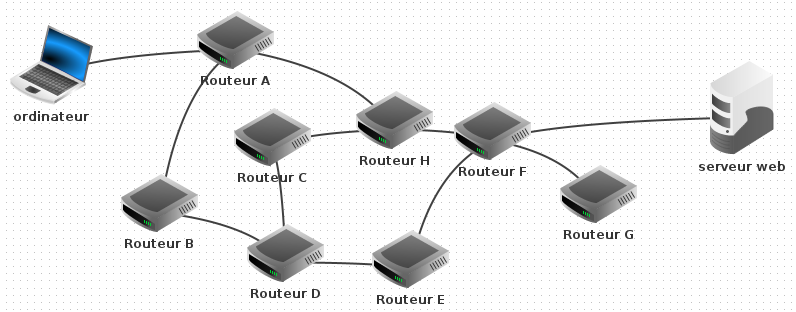
\includegraphics[width=6cm]{ressources/serveur-web.png}
\captionof{figure}{Serveur web}
\label{serveur}
\begin{aretenir}[]
Un \emph{serveur} est une machine accessible en permanence via le réseau Internet. Il est repérable par son \emph{adresse IP}. Il contient des ressources (documents, sites web...) consultables par les internautes.
\end{aretenir}
\end{center}
Les humains retiennent plus facilement une adresse textuelle qu'une adresse IP. 
\begin{aretenir}[]
Une \textbf{URL (Uniform Ressource Locator)} est une adresse textuelle qui identifie un site web. Le \textbf{serveur DNS (Domain Name System)} assure la correspondance: 
\begin{center}
URL $\leftrightarrow$ adresse IP
\end{center}
\end{aretenir}
\begin{center}
\centering
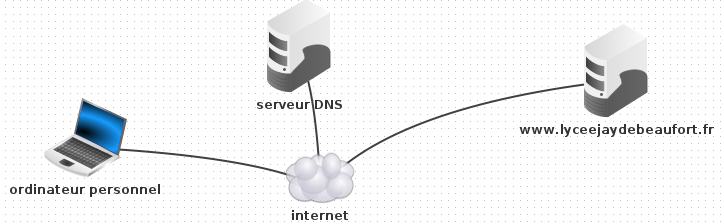
\includegraphics[width=6cm]{ressources/serveur-dns.png}
\captionof{figure}{Serveur DNS}
\label{dns}
\end{center}
\begin{commentprof}
faire le parcours sur le slide
\end{commentprof}
\subsection{Moteurs de recherche}
Quand on ne connaît pas l'URL précise du site qu'on désire visiter, on utilise un \emph{moteur de recherche}.
\begin{itemize}
\item \url{https://duckduckgo.com}
\item \url{https://qwant.com}
\item \url{https://google.com}
\end{itemize}
\begin{aretenir}[]
Un \textbf{moteur de recherche} indexe l'ensemble des pages du web. Il propose des résultats en fonction des \emph{mots-clés} de recherche. Chaque moteur renvoie des résultats différents en fonction de son \textbf{algorithme d'indexation}.
\end{aretenir}
Le \emph{PageRank} est l'algorithme d'analyse des pages web, utilisé par le moteur \emph{Google}.
\begin{center}
\centering
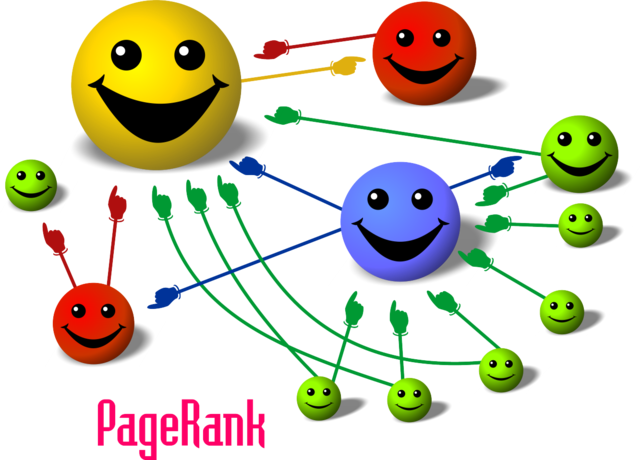
\includegraphics[width=6cm]{ressources/pagerank.png}
\captionof{figure}{Illustration du pagerank}
\label{pagerank}
\end{center}
\begin{commentprof}
score proportionnel au nombre de liens entrants
\end{commentprof}
\section{Sécuriser la connexion}
\subsection{Page web sécurisée}
On repère qu'une page web est sécurisée sur la barre d'adresse du navigateur (figure \ref{https}).
\begin{center}
\centering
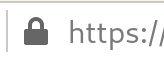
\includegraphics[width=3cm]{ressources/https.png}
\captionof{figure}{Page web sécurisée}
\label{https}
\end{center}
\begin{aretenir}[]
Une page web sécurisée transmet des données \textbf{chiffrées}: si une personne intercepte les informations qui circulent sur le réseau Internet, il ne pourra pas les lire.
\end{aretenir}
\begin{commentprof}
\url{http://jay.info.free.fr} et \emph{Ctrl+Shift+E}
\end{commentprof}
Le \emph{mode privé} d'un navigateur ne garantit pas que les données qui circulent sont chiffrées. Il assure simplement que la page web visitée ne laissera pas de traces sur la machine (historique, cookies...).
\begin{aretenir}[]
Un mot de passe long avec des symboles variés garantit une bonne sécurité.
\end{aretenir}
\subsection{Protection des données}
Les sites web, les réseaux sociaux captent de nombreuses informations de leurs utilisateurs pour ensuite les monnayer.
\begin{center}
\centering
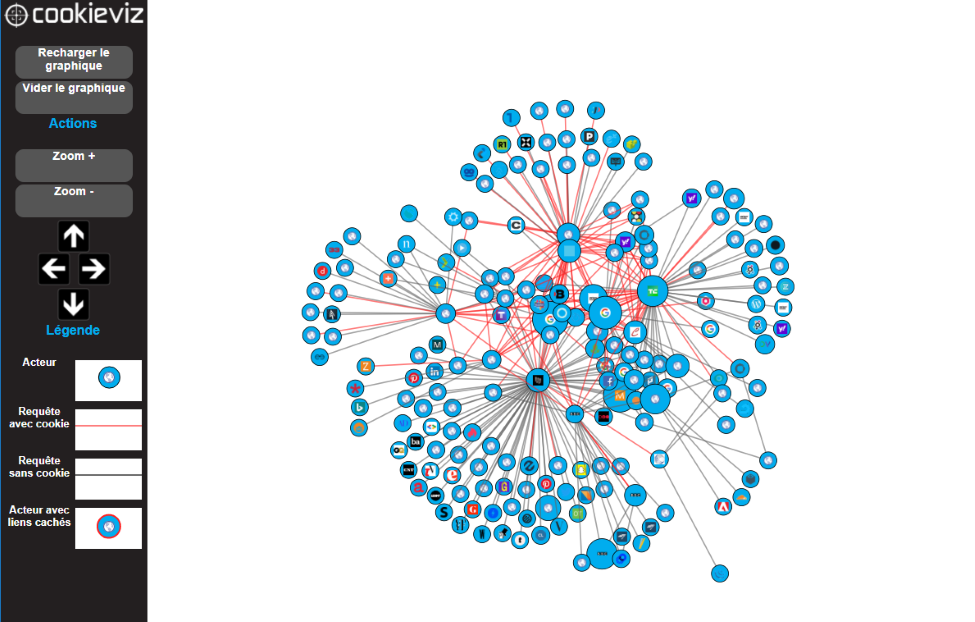
\includegraphics[width=6cm]{ressources/cookieviz.png}
\captionof{figure}{Visualisation des cookies avec CookieViz}
\label{cookieviz}
\end{center}
\begin{aretenir}[]
Un \textbf{cookie} est un fichier texte déposé par le site web, sur l'ordinateur de l'internaute. Il peut contenir de nombreuses informations personnelles (nom, identifiant, date de naissance, géolocalisation...).
\end{aretenir}
L'Europe a mis en place un règlement qui impose aux sites web d'informer les utilisateurs des données collectées et de la possibilité de refuser cette collecte.
\begin{aretenir}[]
Le \textbf{RGPD (Règlement Général pour la Protection des Données)} est adopté par l'Europe en avril 2016 pour une mise en application en mai 2018. Il protège les données de chaque européen.
\end{aretenir}
\end{Form}
\end{document}